\documentclass{ximera}

\graphicspath{{./content/02_5_arclength_function/graphics/}{./graphics/}}

\title{Arclength Function}
\author{Melissa Lynn}
\outcome{Understand and compute the arclength function, and parametrize curves with respect to arclength.}

\begin{document}
\begin{abstract}
\end{abstract}
\maketitle

In our quest to understand the inherent geometry of curves, we've determined how to find the length of a curve. In order to compute the length of a curve, we needed to chose a smooth and simple parametrization for the curve. As it turned out, the length was independent of this choice of parametrization, so we didn't need to worry about different parametrizations yielding different lengths.

Looking ahead in our study of the inherent geometry of curves, we would like to find a way to quantify how ``curvy'' a curve is. In order to do this, we'll need a standardized parametrization, to avoid getting different measures of curviness for different parametrizations. This special parametrization will be one that traverses the path at a constant speed of $1$. In order to define this parametrization, we again turn our attention to arclength, this time defining a function that computes arclength at varying points on a curve. We will later see how the arclength function can be used to find the standardized parametrization which we require.

\section*{The Arclength Function}

Suppose we're considering the arclength of some curve $\vec{x}(t)$. Let's fix some starting point at time $t=a$, but instead of fixing the endpoint as well, we'll let that vary, so we'll think of it as a variable. For each choice of endpoint, we can compute the arclength along the curve from our fixed start point to the endpoint. This gives us a special function, which we call the \emph{arclength function}:
\[
s(t) = \int_a^t \|\vec{x}'(\tau)\|d\tau.
\]
Note that we're using $\tau$, pronounced ``tau,'' for the variable of integration, to avoid confusion with the $t$ used for the endpoint. We'll commonly use $s$ to denote arclength, often omitting the variable $t$.

\begin{image}
\begin{tikzpicture}
%\draw plot [thick, smooth, tension=.6] coordinates {(0,0) (1,1.312) (2, 1.5) (3,.937) (4,0) (5,-.937) (6, -1.5) (7, -1.312) (8,0)};
\draw [thick, blue]         (0,0) to[out=-30,in=210] (2,2);
\draw  (2,2) to[out=30,in=180] (5,4);
\draw  (5,4) to[out=0,in=210]   (8,0);
\filldraw (0,0) circle[radius=1pt];
\node[above left] at (0,0) {$\vec{x}(a)$};
\filldraw (8,0) circle[radius=1pt];
\node[above right] at (8,0) {$\vec{x}(b)$};
\filldraw[blue] (2,2) circle[radius=1pt];
\node[above left] at (2,2) {$\vec{x}(t)$};
\node[below right] at (1,1) {\color{blue} $length = \int_a^t \|\vec{x}'(\tau)\|d\tau$};
\end{tikzpicture}
\end{image}

Let's see what happens when we differentiate the arclength function. First, recall part of the Fundamental Theorem of Calculus: if $f$ is a continuous function, and we define $F(x) = \int_a^x f(u)\;du$, then
\[
F'(x) = \answer{f(x)}.
\]
Applying this to the arclength function, $s(t) = \int_a^t \|\vec{x}'(\tau)\|\;d\tau$, we have
\[
s'(t) = \|\vec{x}'(t)\|.
\]
This means that the derivative of the arclength function is the \emph{speed} of the parametrization, or the speed of a particle moving along the path. If we remember that the arclength function is computing the distance traveled along the path, it makes sense that its derivative should be speed.


\section*{Parametrization with Respect to Arclength}

One of the most important uses of the arclength function is to reparametrize a curve according to \emph{arclength}. This means that we find a special parametrization $\vec{x}(s)$ for $0\leq s\leq L$, where $L$ is the length of the curve. This parametrization has the property that $\vec{x}(s)$ is always the point distance $s$ along the curve.

\begin{image}
\begin{tikzpicture}
%\draw plot [thick, smooth, tension=.6] coordinates {(0,0) (1,1.312) (2, 1.5) (3,.937) (4,0) (5,-.937) (6, -1.5) (7, -1.312) (8,0)};
\draw [thick, blue]         (0,0) to[out=-30,in=210] (2,2);
\draw  (2,2) to[out=30,in=180] (5,4);
\draw  (5,4) to[out=0,in=210]   (8,0);
\filldraw (0,0) circle[radius=1pt];
\node[above left] at (0,0) {$\vec{x}(a)$};
\filldraw (8,0) circle[radius=1pt];
\node[above right] at (8,0) {$\vec{x}(b)$};
\filldraw[blue] (2,2) circle[radius=1pt];
\node[above left] at (2,2) {$\vec{x}(s)$};
\node[below right] at (1,1) {\color{blue} $length = s$};
\end{tikzpicture}
\end{image}

We'll see that the arclength parametrization is very useful for understanding the geometry of a curve, but unfortunately it is often computationally difficult to find. The process for reparametrizating with respect to arclength is:
\begin{enumerate}
\item Find a parametrization $\vec{x}(t)$ for the curve.
\item Find the arclength function $s(t)$.
\item Invert the arclength function. That is, write the parameter $t$ in terms of the arclength $s$.
\item Substitute the expression for $t$ into the original parametrization $\vec{x}(t)$, which gives you a parametrization for the curve with respect to arclength, $s$.
\end{enumerate}

These steps sound simple enough, but are complicated by the fact that arclength integrals rarely simplify nicely, so it can be difficult to write down an inverse. Below, we work through an example where arclength can be simplified nicely.

\begin{example}
Consider the helix $\vec{x}(t) = (3\cos(t), 3\sin(t), 4t)$ for $0\leq t \leq 8\pi$. We'll reparametrize this helix with respect to arclength.

\begin{image}
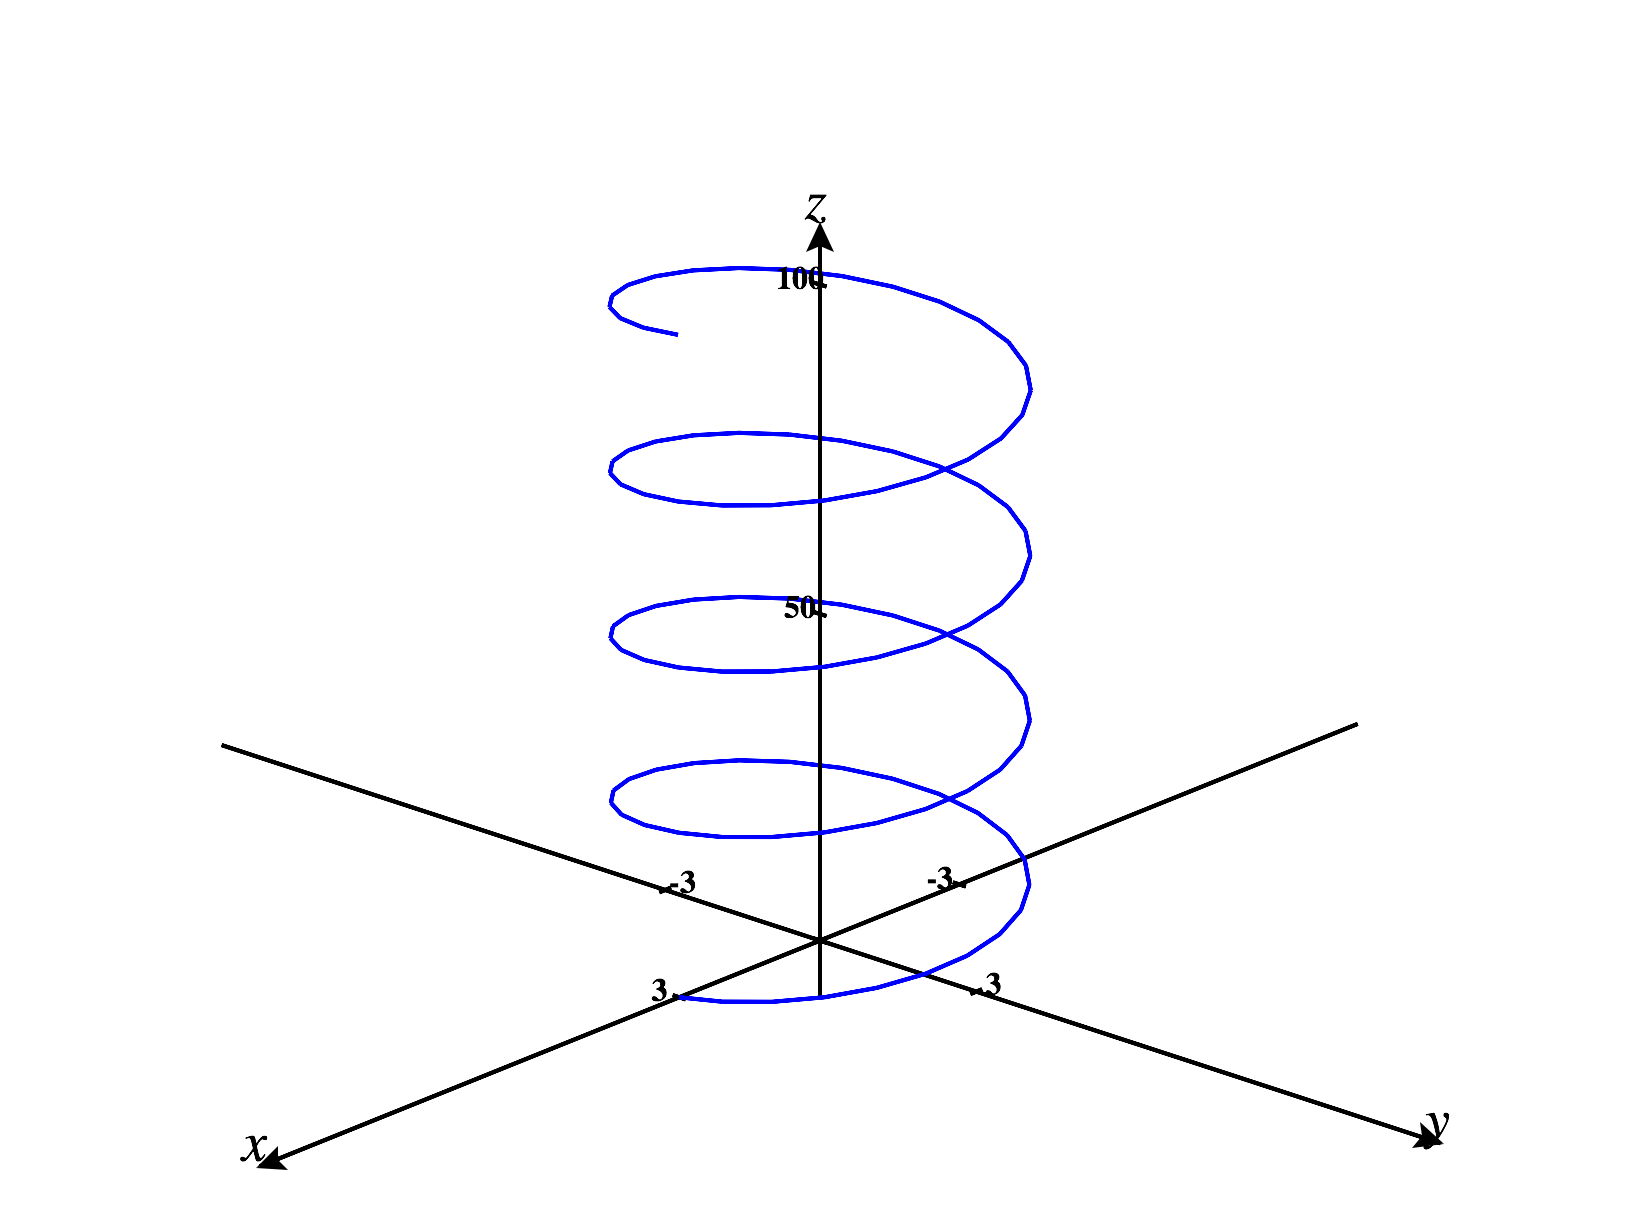
\includegraphics[width = \textwidth]{CalcPlot3D-arclength_ex}
\end{image}

We're already given a parametrization for the curve, so we'll begin by finding the arclength function $s(t) = \int_0^t \|\vec{x}'(\tau)\|\;d\tau$. First, we'll find the velocity.
\[
\vec{x}'(t) = \answer{(-3\sin(t),3\cos(t), 4)} 
\]
Then, we can find the speed.
\[
\|\vec{x}'(t)\| = \answer{5}
\]
Now, we find the arclength function by integrating speed.
\begin{align*}
s(t) &= \int_0^t \|\vec{x}'(\tau)\|\;d\tau\\
&= \int_0^t 5d\tau\\
&= \answer{5t}
\end{align*}
We now find the inverse of the arclength function, to find the parameter $t$ in terms of arclength $s$. Working from $s=5t$, we have
\[
t = \answer{s/5}.
\]
We substitute this into our original parametrization, and we have
\[
\vec{x}(s) = \answer{(3\cos(s/5), 3\sin(s/5), \frac{4}{5}s)}.
\]
This gives us the parametrization with respect to arclength.
\end{example}

We will soon see that the arclength parametrization can be used to examine the inherent geometry of the curve, independent of how quickly or slowly a given path traverses the curve. This is because the arclength parametrization always has unit speed. Let's investigate why this is true.

Let's suppose we obtain the arclength parametrization $\vec{x}(s)$ from some parametrization $\vec{x}(t)$. Since $s$ is a function of $t$, we can use the chain rule to find the velocity of $\vec{x}(t)$. In particular,
\[
\vec{x}'(t) = \vec{x}'(s)\cdot s'(t).
\]
Earlier, we found that $s'(t) = \|\vec{x}'(t)\|$. Substituting, we have
\[
\vec{x}'(t) = \vec{x}'(s)\|\vec{x}'(t)\|.
\]
Taking the magnitude of both sides, we have
\[
\|\vec{x}'(t)\| = \|\vec{x}'(s)\|\cdot \|\vec{x}'(t)\|.
\]
From this, we see that
\[
\|\vec{x}'(s)\| = 1.
\]
So, the speed of the arclength parametrization is always 1.

\textit{Images were generated using \href{https://www.monroecc.edu/faculty/paulseeburger/calcnsf/CalcPlot3D/}{CalcPlot3D}.}

\end{document}